\section{Introducción}   %revisaaaaaaaaaaaaaarrrrrrr
\noindent La finalidad de esta práctica es obtener la dureza del agua mediante una serie de reacciones donde el primer proceso nos dará el volumen de calcio y magnesio presente en el agua (del grifo) y el segundo proceso nos dará sólo el volumen del magnesio, que nos permitirá calcular la cantidad de calcio presente en el agua, para así poder volver a la primera parte y calcular la cantidad de magnesio. Con estas dos magnitudes seremos capaces de calcular lo que nos pide la práctica: la dureza del agua. A lo largo de esta práctica nos va a ser útil conocer qué significan los distintos colores que vamos a obtener:

\begin{multicols}{3}
    $pH < 7$ ~\rightsquigarrow ~ rojo vino
    
    \vspace{0.1cm}
    
    $7 < pH < 11.5$ ~\rightsquigarrow ~ azul
    
    \vspace{0.1cm}
    
    $pH > 11.5$ ~\rightsquigarrow ~ naranja
\end{multicols}

\section{Inventario}  
\noindent En esta práctica contamos con:
\begin{multicols}{2}
    \begin{itemize}
        \item 2 erlenmeyer
        \item 3 vasos de precipitados
        \item Un embudo Büchner
        \item Un matraz kitasatos
        \item Un embudo
        \item Una varilla
        \item Una espátula
        \item Una pipeta 
        \item Una bureta
        \item Una placa calefactora
        \item Unos guantes de silicona
        \item Amoniaco ($NH_3$)
        \item Indicadores: Rojo de metilo y Negro de eriocrom T
        \item Oxalato de sodio ($C_2Na_2O_4$)
        \item Ácido clorhídrico (HCl)
    \end{itemize}
\end{multicols}

\begin{figure}[H]
    \centering
    \hspace*{-3cm}
        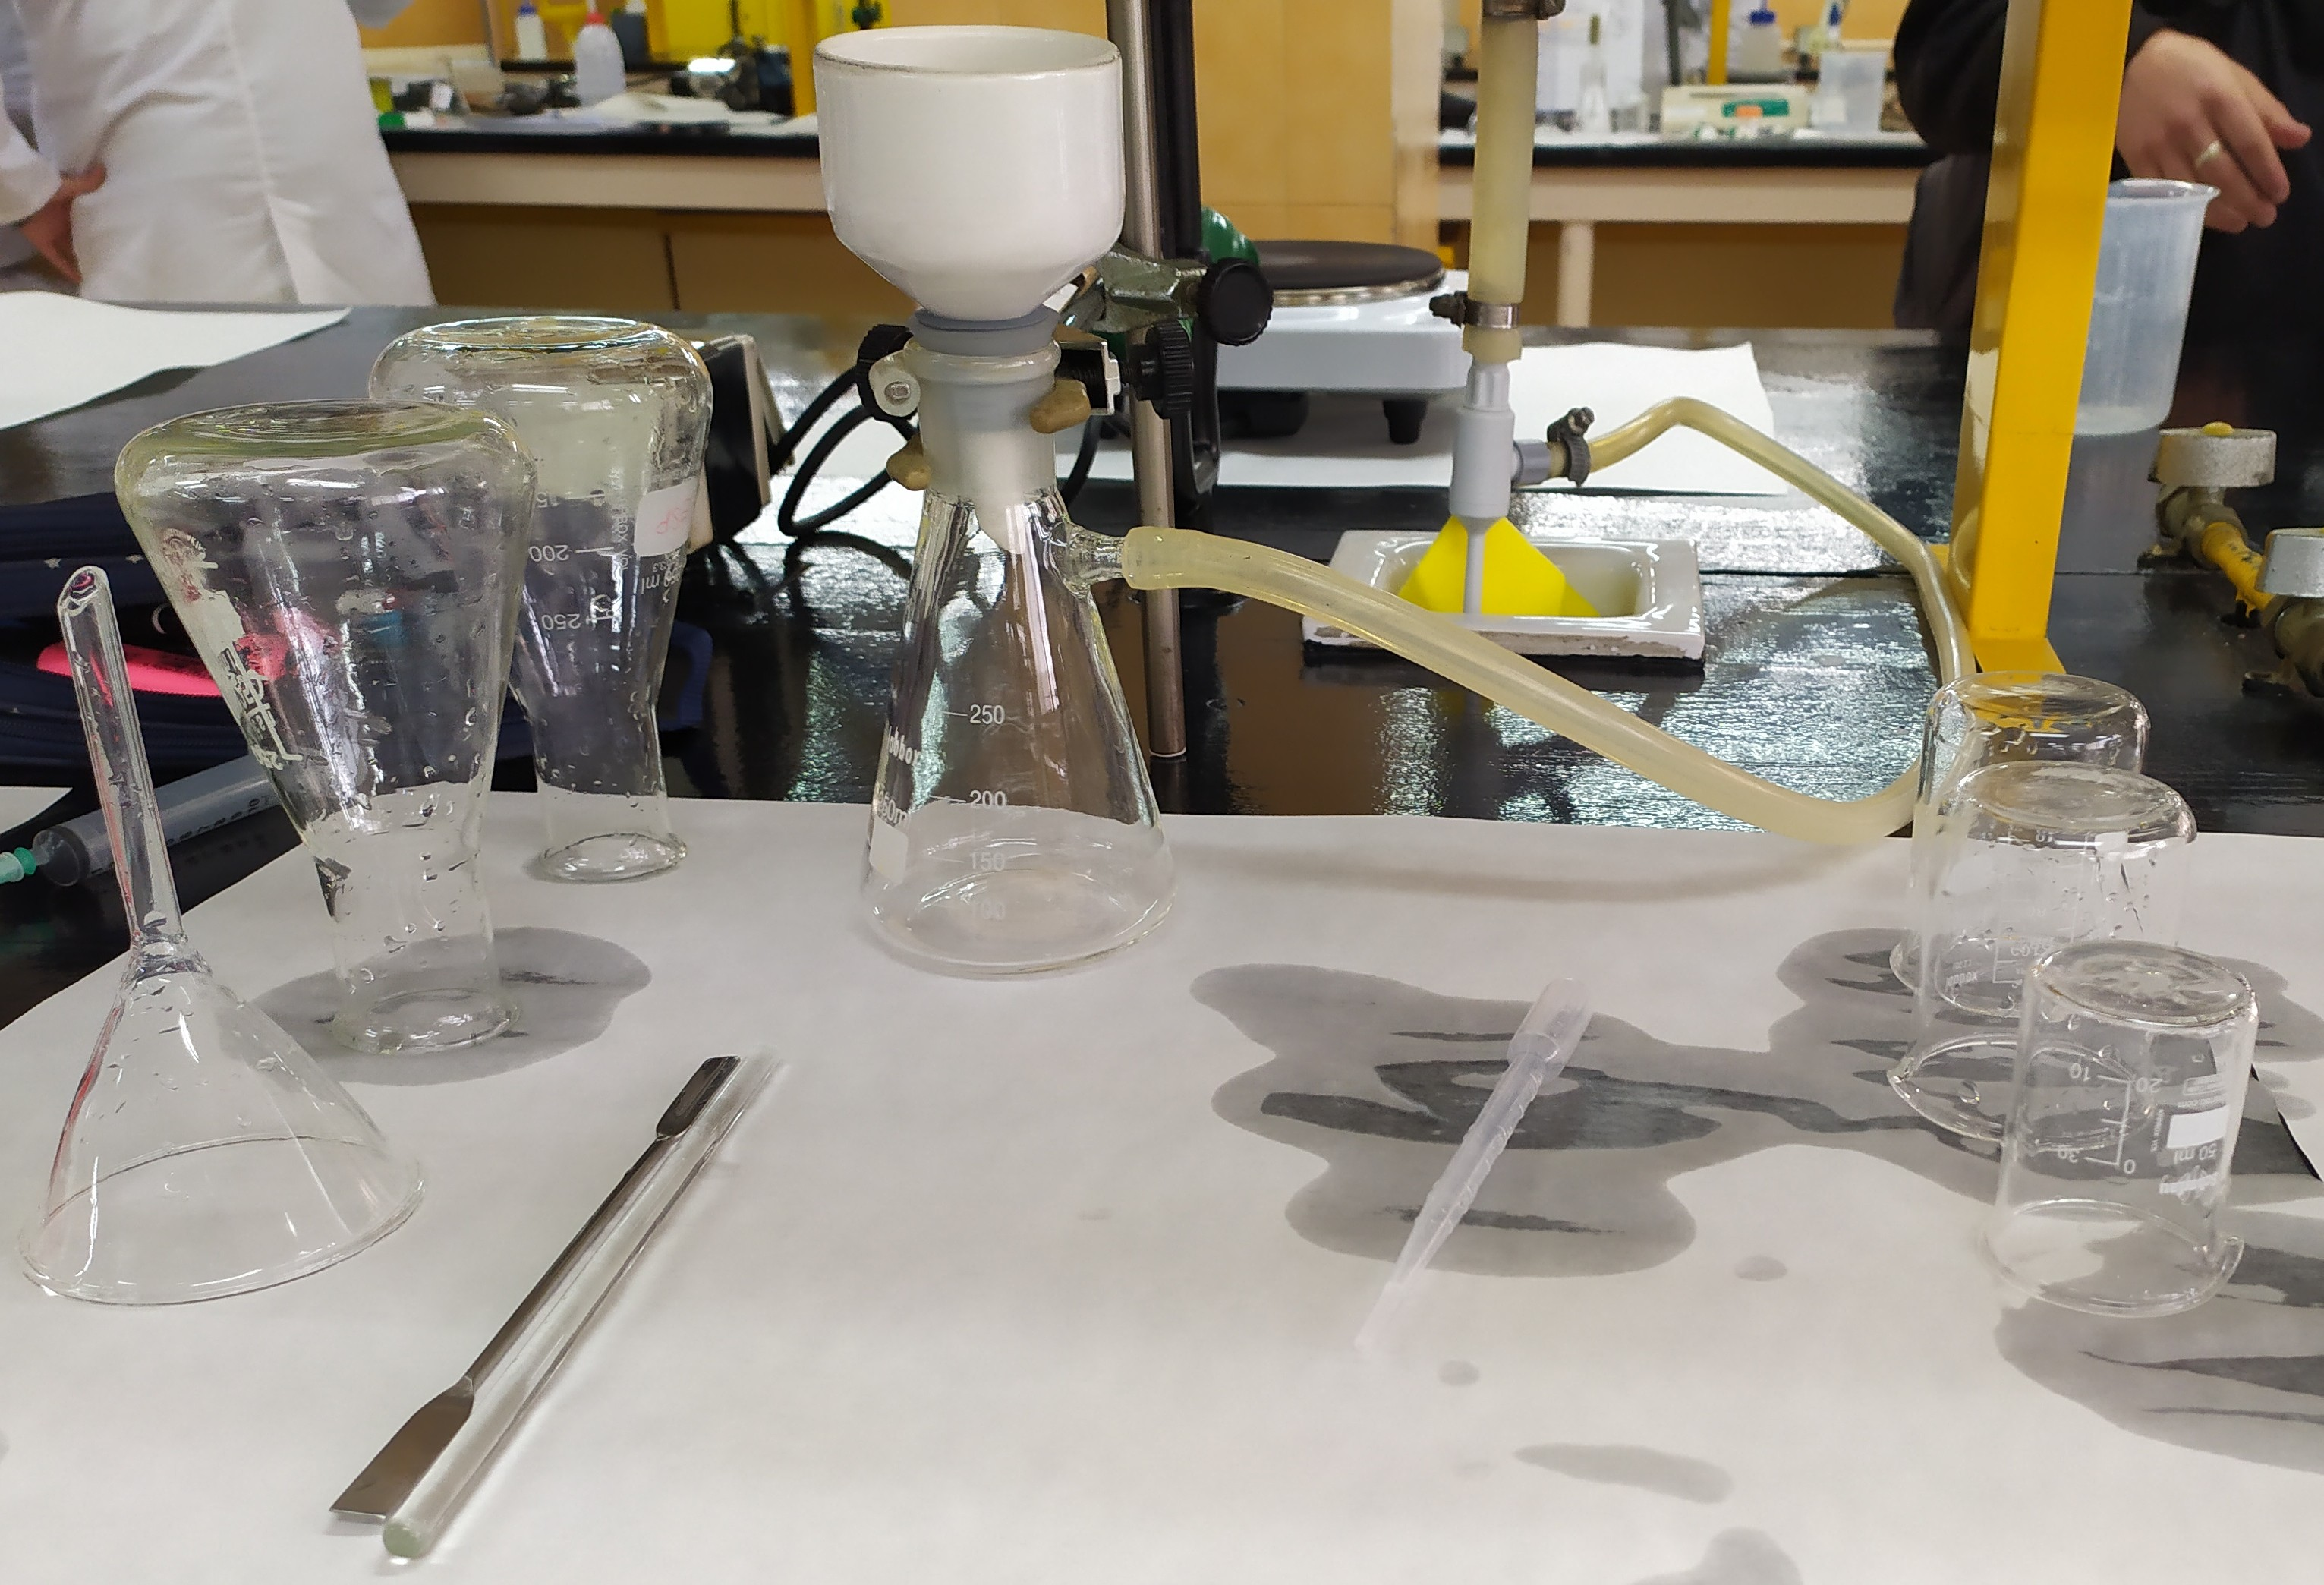
\includegraphics[scale = 0.049]{fotos/set4.jpg}
        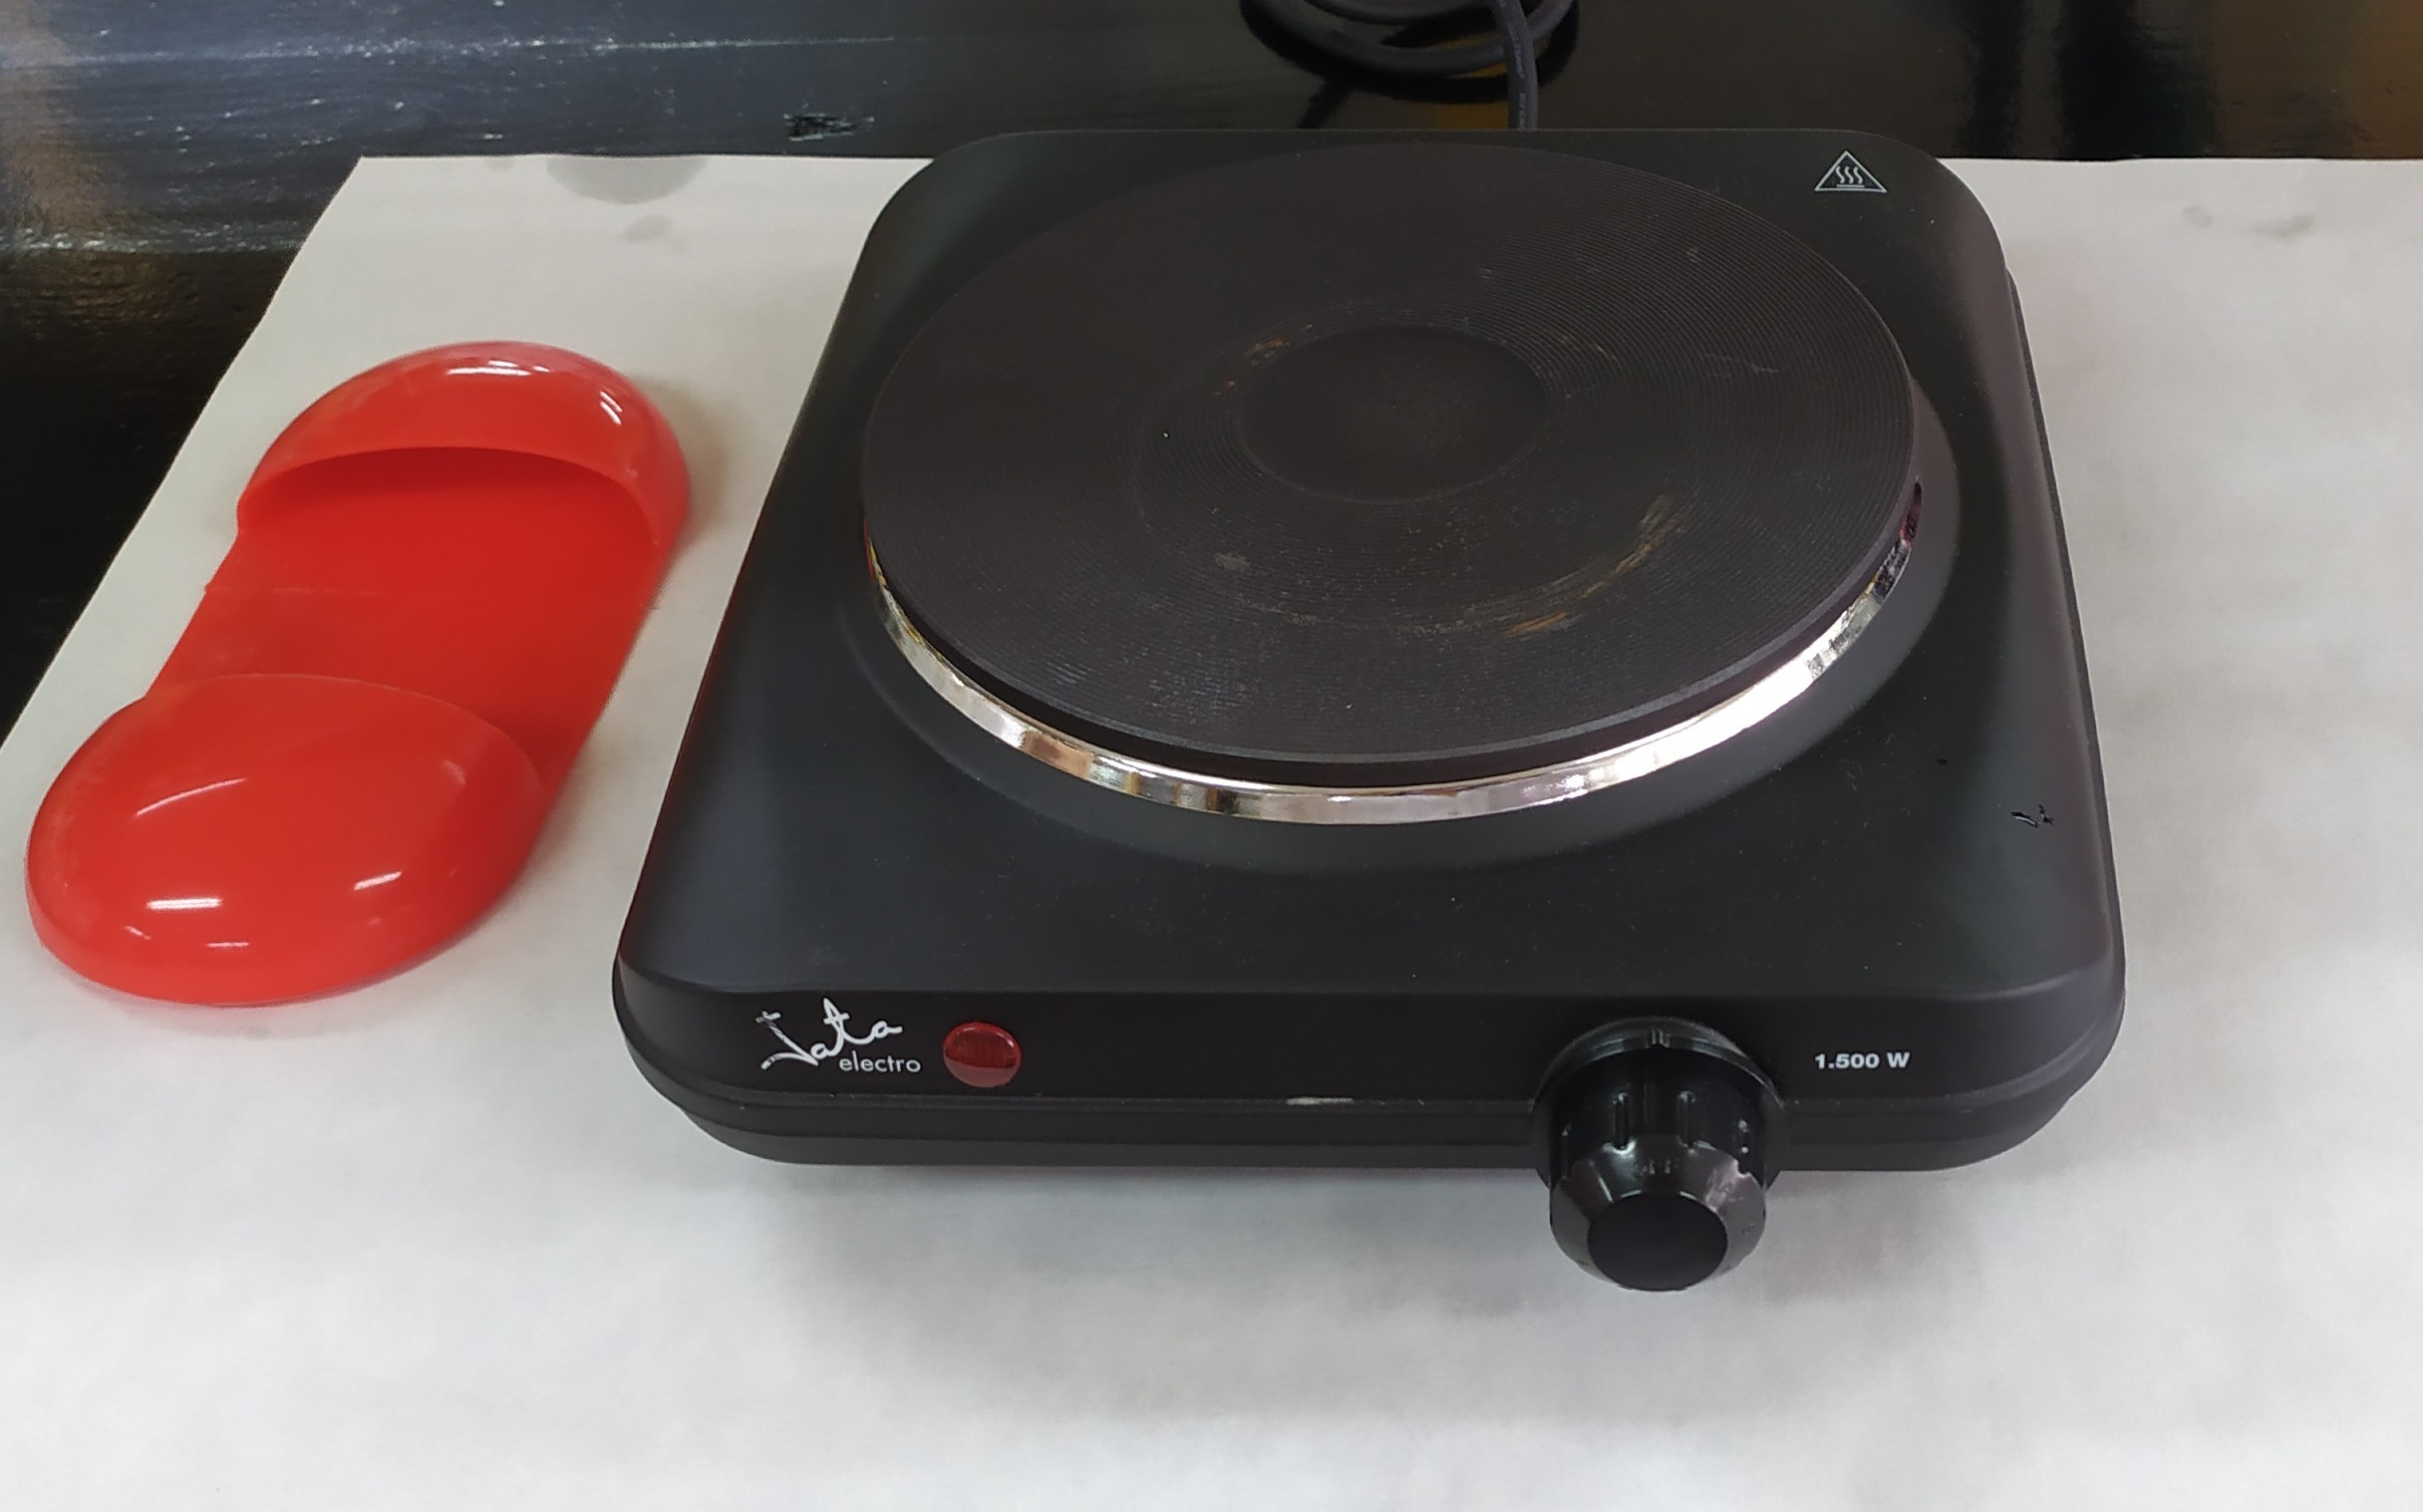
\includegraphics[scale = 0.0673]{fotos/placa4.jpg}
        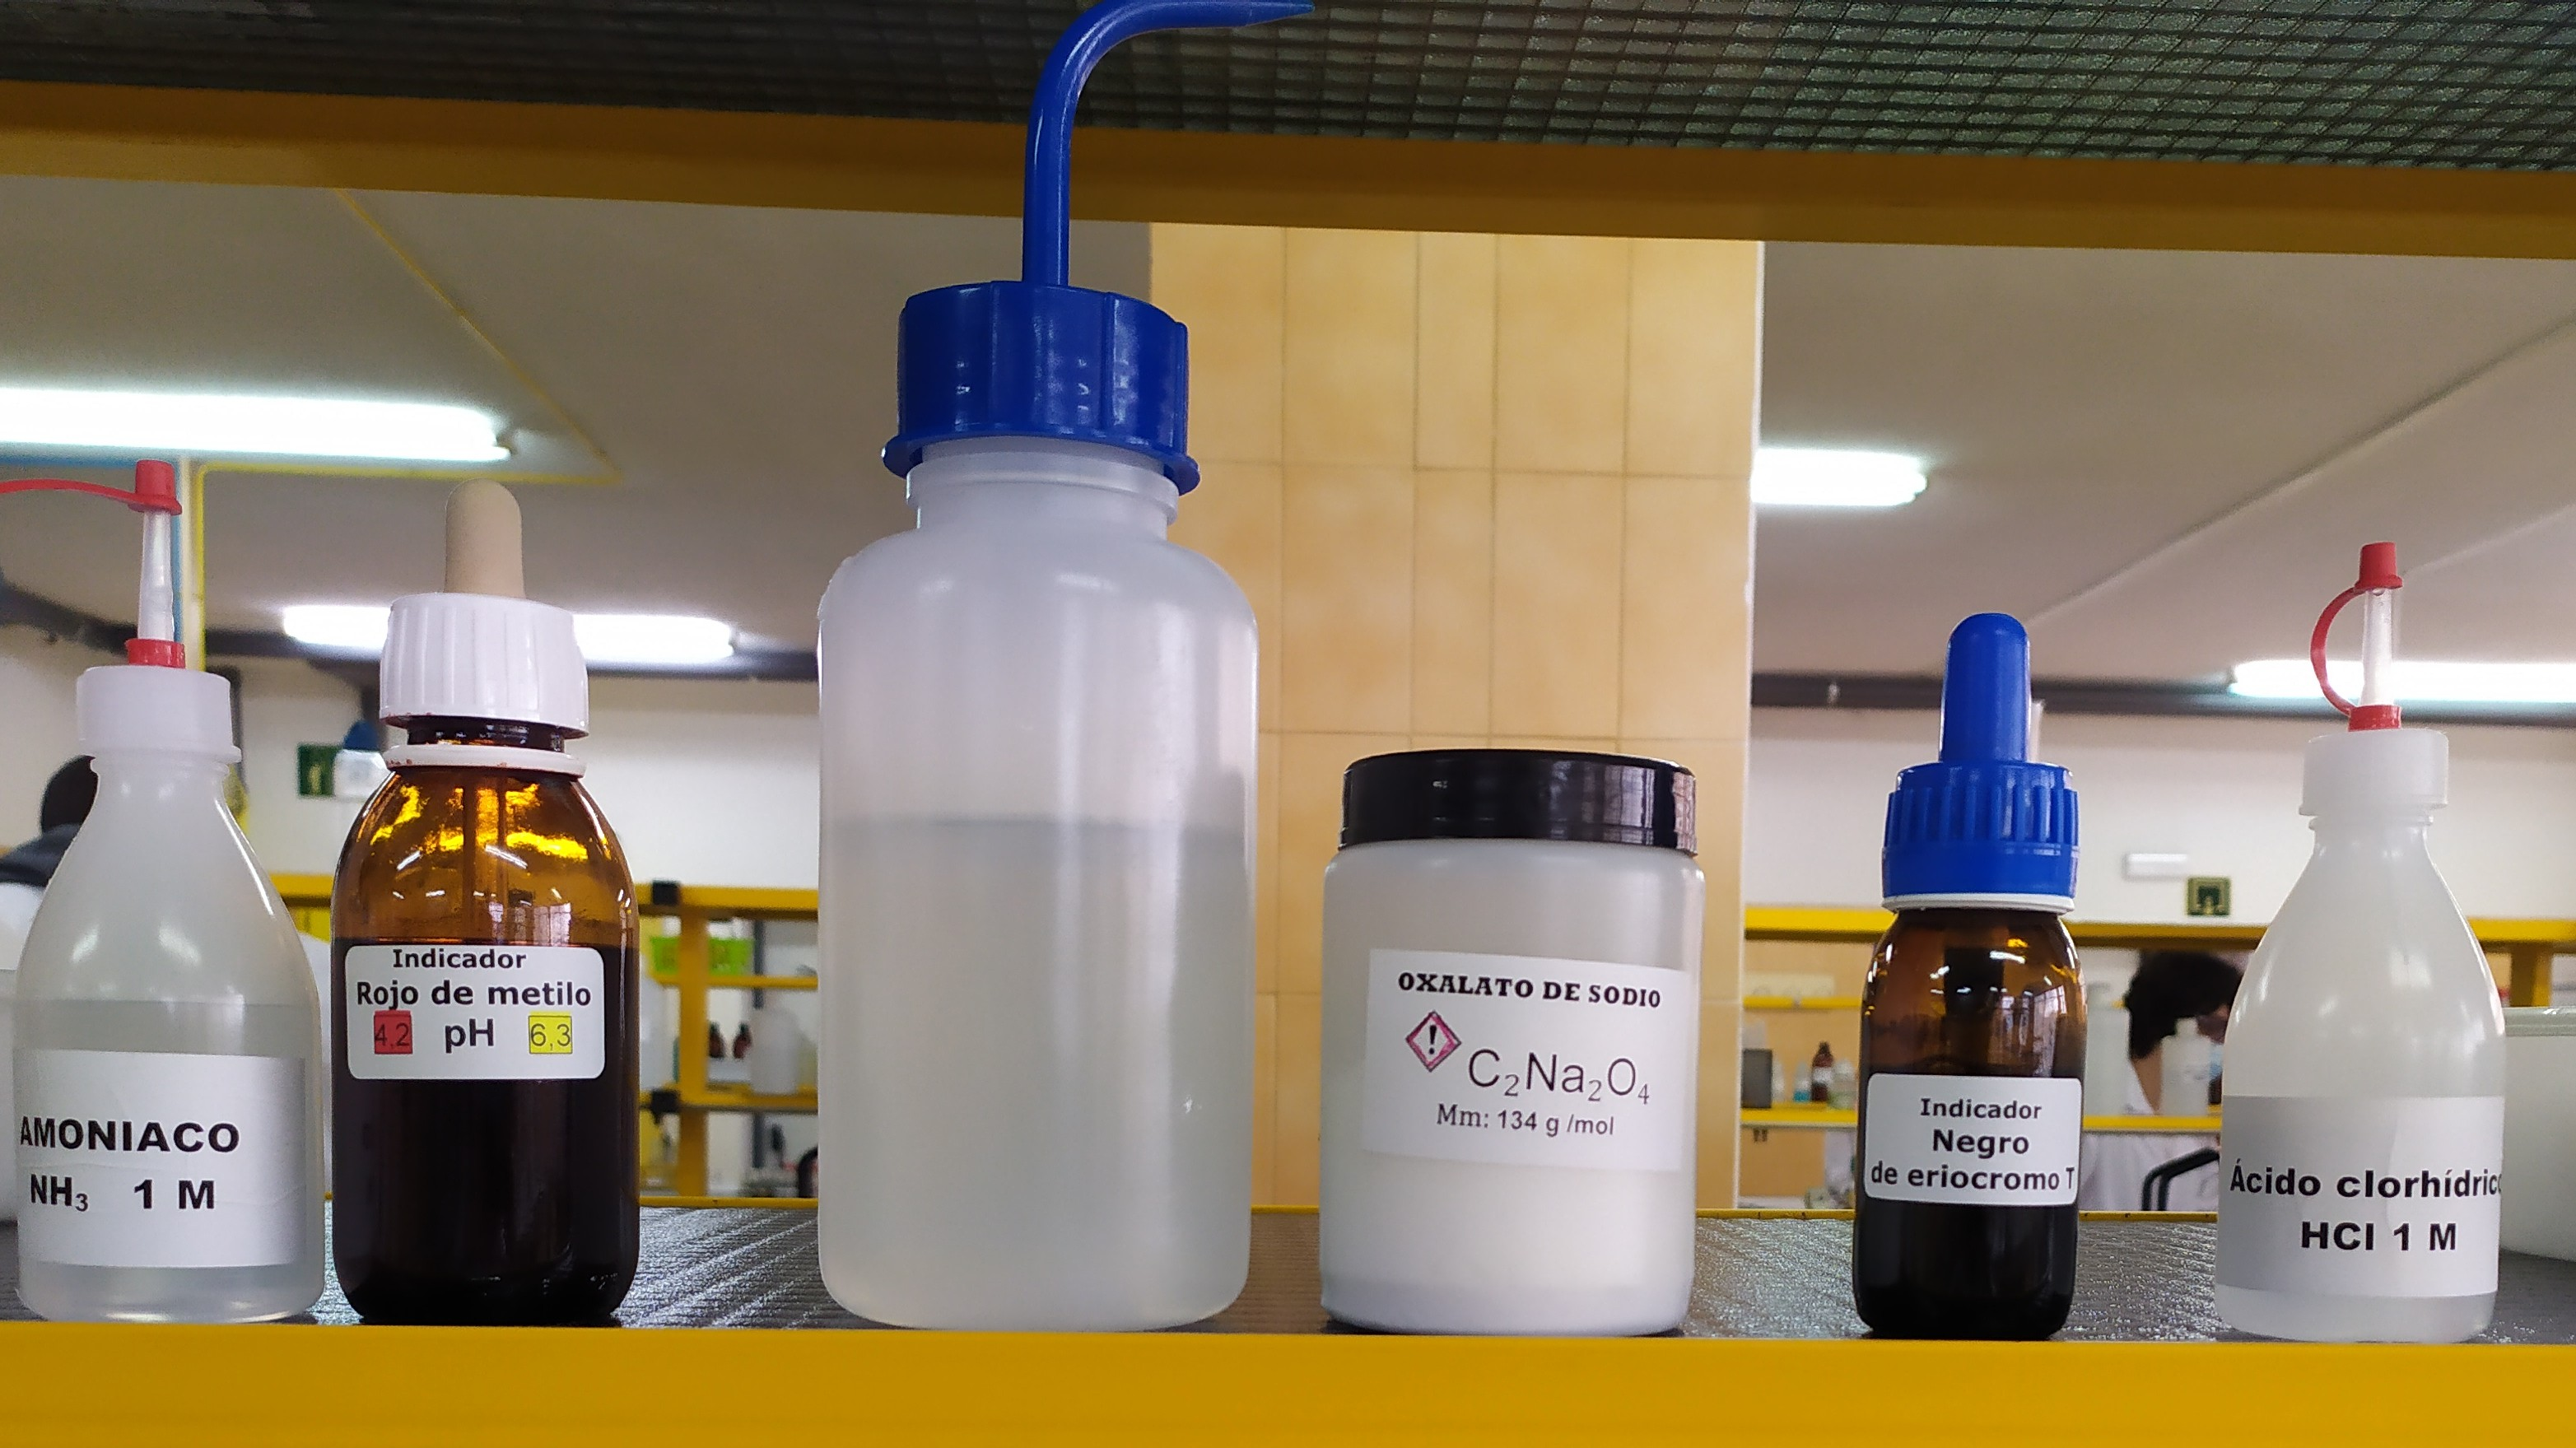
\includegraphics[scale = 0.058]{fotos/liqui4.jpg}
    \hspace*{-3cm}
    \caption{Material descrito}
\end{figure}
\vspace{-3cm}
\clearpage

\section{Procedimiento}
\noindent Esta práctica consta de dos partes, en la primera determinamos la dureza total del agua, y en la segunda la dureza específica magnésica y cálcica. Y para determinar dicha dureza usaremos el agua del grifo.

\vspace{0.2cm}

\noindent En la \textcolor{red}{primera parte} mediremos con un matraz aforado $100 mL$ de agua, lo pasamos a un erlenmeyer donde añadimos unas 10 gotas de rojo metilo hasta obtener un color amarillo y luego acidificamos la disolución añadiendo gotas de \ce{HCl} $1M$ hasta que se forme un color rosado; en nuestro caso hemos necesitado alrededor de 8 gotas. Y puesto que hay que repetir el proceso 3 veces, vamos a usar 3 matraces erlenmeyer y lo haremos simultáneamente. Por ello, una vez tenemos las tres disoluciones, las calentamos hasta que comiencen a hervir para después de que se enfríen,  neutralizar con 10 gotas de \ce{NaOH} hasta volver al color amarillo (indicador de un pH $\approx$ 7).

\vspace{0.2cm}

\noindent A continuación, añadimos 2 mL de tampón $NH_4^+/NH_3$ y entre 6 y 8 gotas de negro eriocromo T hasta obtener un color rojo vino (pH $\approx$ 10). Mientras, llenamos la bureta con EDTA (0.001M) para valorar la muestra. Vamos a ver qué cantidad de volumen de EDTA es necesario para que nuestra muestra cambie de ese color rojo vino a un color azul. Ese volumen nos indicará la cantidad de calcio y magnesio que hay en el agua. 

\begin{multicols}{3}
\vspace{0.3cm}

$V_1$ = 35.2 mL

\vspace{0.1cm}

$V_2$ = 36 mL

\vspace{0.1cm}

$V_3$ = 34.7 mL

\vspace{0.3cm}
\end{multicols}

\noindent Estos volúmenes nos servirán para el apartado \ref{cuest}.

\vspace{0.2cm}

\noindent En la \textcolor{red}{segunda parte} repetiremos el proceso de medir 3 veces 100 mL de agua y le añadiremos unas 5-6 gotas de rojo metilo hasta encontrar el color amarillo, para luego añadirle HCl y pondremos en una punta de espátula oxalato sódico hasta obtener un color rosado. 

\vspace{0.1cm}

\noindent Volvemos a hervir las tres mezclas para eliminar los carbonatos, las enfríamos y después las neutralizamos con $NH_3$(1M) hasta tener un color amarillo. Seguidamente, esperaremos unos 10 minutos para que precipite el oxalato de calcio. Posteriormente, filtramos la disolución para retirar el precipitado. 

\vspace{0.1cm}

\noindent Tras este proceso, adicionamos 5 mL del tampón $NH_4^+/NH_3$ y unas 20 gotas de negro eriocromo T hasta obtener un rojo vino. 

\vspace{0.1cm}

\noindent Subsiguientemente, volvemos a llenar la bureta de EDTA y volvemos a medir el volumen gastado cuando cambie de color.

\vspace{-0.2cm}
\begin{multicols}{3}
\vspace{0.3cm}

$V_1$ = 15.5 mL

\vspace{0.1cm}

$V_2$ = 17 mL

\vspace{0.1cm}

$V_3$ = 16.9 mL

\vspace{0.3cm}
\end{multicols}

\noindent Estos volúmenes nos servirán para el apartado \ref{cuest}.


\clearpage
\section{Cuestiones}\label{cuest}   

\noindent\textcolor{BlueViolet}{\textbf{\textit{Cuestiones a y b:}}}


\noindent En este apartado nos piden calcular la dureza tanto del Magnesio como del Calcio.

-- Con los volúmenes obtenidos en la primera parte podemos calcular la dureza total (EDTA: 0.01M):

\[V_1 = 35.2 mL \rightsquigarrow 0.0352 L \cdot \frac{0.01 mol}{1 L} = 3.52\cdot{10^{-4}} moles de EDTA  \rightsquigarrow 3.52\cdot{10^{-3}} M  (\ce{Mg}^{+2} + \ce{Ca}^{+2}\]

\[V_2 = 36 mL \rightsquigarrow 0.036 L \cdot \frac{0.01 mol}{1 L} = 3.6\cdot{10^{-4}} moles de EDTA  \rightsquigarrow 3.6\cdot{10^{-3}} M  (\ce{Mg}^{+2} + \ce{Ca}^{+2}\]

\[V_3 = 34.7 mL \rightsquigarrow 0.0347 L \cdot \frac{0.01 mol}{1 L} = 3.47\cdot{10^{-4}} moles de EDTA  \rightsquigarrow 3.47\cdot{10^{-3}} M (\ce{Mg}^{+2} + \ce{Ca}^{+2}\]

\noindent Y la media de los tres tiene un valor de: $3.53\cdot{10^{-3}} M (Mg^{+2} + Ca^{+2})$

\vspace{0.3cm}

-- Ahora, con los volúmenes obtenidos en la segunda parte podemos calcular la dureza del magnesio:

\[V_1 = 15.5 mL \rightsquigarrow 0.0155 L \cdot \frac{0.01 mol}{1 L} = 1.55\cdot{10^{-4}} moles de EDTA  \rightsquigarrow 1.55\cdot{10^{-3}} M (\ce{Mg}^{+2}\]

\[V_2 = 17 mL \rightsquigarrow 0.017 L \cdot \frac{0.01 mol}{1 L} = 1.17\cdot{10^{-4}} moles de EDTA  \rightsquigarrow 1.17\cdot{10^{-3}} M (\ce{Mg}^{+2}\]

\[V_3 = 16.9 mL \rightsquigarrow 0.0169 L \cdot \frac{0.01 mol}{1 L} = 1.69\cdot{10^{-4}} moles de EDTA  \rightsquigarrow 1.69\cdot{10^{-3}} M (\ce{Mg}^{+2}\]


\noindent Y la media de los tres tiene un valor de: \underline{$1.65\cdot{10^{-3}} M (Mg^{+2})$}

\vspace{0.2cm}

-- Por último, calculamos la dureza del Calcio:
\[ [Ca^{+2}] =  3.53\cdot{10^{-3}} M (\ce{Mg}^{+2} + Ca^{+2}) - 1.65\cdot{10^{-3}} M (\ce{Mg}^{+2}) = 1.88\cdot{10^{-3}} M (\ce{Ca}^{+2})\]

\noindent Los valores obtenidos concuerdan con los valores en mg/l de $CaCO_3$

\clearpage

\noindent\textcolor{BlueViolet}{\textbf{\textit{c) Indique algún método por el que pudiéramos hallar experimentalmente la dureza cálcica.}}}


\vspace{0.1cm}

\noindent Para hallar experimentalmente la dureza cálcica experimentalmente tendríamos que sustituir el indicador eriocromo T por 'murexida'. Y usaríamos hidróxido sódico para aumentar el pH y para que bloquee los iones de calcio que hay en la muestra.

\vspace{0.3cm}

\noindent De este modo, obtendríamos una disolución rosada, y en este momento mediríamos el volumen gastado de EDTA, lo que nos permitiría calcular la dureza del calcio como hicimos con el magnesio.







